\documentclass{llncs}
\usepackage{fullpage}

%load needed packages
\usepackage{graphicx}
\usepackage{array}
\usepackage{booktabs}
\usepackage[utf8]{inputenc}
\usepackage{amsmath} 
\usepackage{hyperref}


\begin{document}

\title{Task B}
\subtitle{Comparative Analysis of Methods in Supervised Learning and Deep Learning}

\author{Diego De Pablo}
\institute{\email{depablodiego@uma.es} \\
Health Engineering. Málaga University.}

\maketitle 

\vspace{1cm} % Space down the title

\textit{
	This work explores supervised learning methodologies with a focus on deep learning (DL). We discuss the importance of splitting datasets into training and test sets, as well as cross-validation techniques for model evaluation. Further, we examine artificial neural networks (ANNs) and the advancements of DL over traditional neural networks, emphasizing innovations like convolutional layers and recurrent networks. Case studies of DL applications, such as AlphaFold in protein folding and DeepMind's AI in medical imaging, are also highlighted. Additionally, we address challenges such as overfitting and data limitations in biomedical fields. All this theoretically.}



\section{Introduction}

In the rapidly evolving field of machine learning, supervised learning and deep learning have emerged as powerful solutions for complex problems across various domains. Supervised learning involves training models on labeled data to make predictions about unseen data, and it has been widely applied in tasks like classification and regression. Deep learning, a subset of machine learning, which focuses on using multi-layered artificial neural networks to process large volumes of data and automatically extract complex features. These networks, known as deep neural networks, are composed of several hidden layers between the input and output, allowing them to learn hierarchical representations of the data. \cite{Goodfellow}

Unlike traditional machine learning algorithms, where the relevant features are often designed manually, in deep learning deep neural networks are able to learn these features directly from raw data, such as images, audio or text.\cite{Goodfellow}

One of the critical challenges in developing machine learning models is establishing a fair comparison between different methods. This ensures that models are evaluated accurately, enabling practitioners to select the best model for their specific problem. To achieve this, it is crucial to carefully choose appropriate metrics from the literature and follow standardized procedures for training and testing.\cite{LeCun2015}

Through this study, it seek to gain a deeper understanding of supervised learning, explore critical aspects of model evaluation, and appreciate the transformative potential of deep learning in solving complex, real-world problems.


\section{Supervised Learning Methodology}

The report will address a number of key questions related to supervised methods and deep learning (DL). Starting with an introduction to supervised learning methodology, it will discuss the importance of splitting data into training and test sets to avoid generalization and model overfitting issues. Then, it will explore the concept of cross-validation, a technique that improves model performance evaluation and prevents overfitting by using different subsets of the data for training and validation.

Next, it will delve into artificial neural networks, a fundamental component of machine learning, and how deep neural networks (DL) go beyond traditional forward propagation networks. It will discuss what distinguishes deep learning models, exploring their advanced capabilities compared to classical neural networks.

In addition, it will present some notable cases where companies such as Google have achieved surprising results using DL in different domains, such as protein structure prediction or medical image analysis. A crucial challenge in training DL models, overfitting, will also be discussed, and how deep networks employ techniques such as regularization and dropout to mitigate this problem.

Finally, the limitations that lack of data presents in the application of DL models, especially in the biomedical field, will be examined, and available techniques, such as transfer learning and synthetic data generation, will be reviewed to overcome this barrier and improve the applicability of these models in contexts where data is scarce.

\subsection{About Supervised Learning Methodology}

Supervised learning is a type of machine learning where a model is trained using labeled data, meaning that each training example is paired with the correct output. The goal of supervised learning is to learn a mapping from inputs to outputs so that the model can make accurate predictions when given new, unseen data.\cite{Hastie2009}


For example if you have a dataset of medical records where each record includes features like age, blood pressure, and cholesterol levels (inputs) along with whether or not the patient has a disease (output), a supervised learning algorithm could be trained on this data to predict whether a new patient is at risk of the disease.

\subsubsection{Key Concepts in Supervised Learning:}

\textit{Why do we need to split the dataset into training and test sets?}

When developing a supervised learning model, it is crucial to divide the dataset into training and test sets. The training set is used to train the model, meaning the model learns from this subset of data by adjusting its parameters to minimize errors in predictions. The test set, on the other hand, is used to evaluate the model's performance on data it has never seen before. This separation ensures the model's ability to generalize to new, unseen data, which is essential for robust performance in real-world scenarios.

You can see the figure \ref{fig:dataset} where you can see how a dataset is normally treated when applying a supervised method.

\vspace{-20pt} % Ajusta este valor para reducir el espacio

\begin{figure}[h!]
	\begin{center}  % Usamos el entorno 'center'
		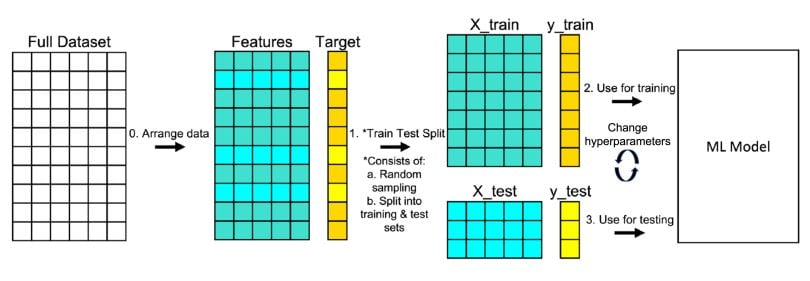
\includegraphics[width=1\textwidth]{images/dataset.jpg}
		\caption{Train test split procedure. | Image: Michael Galarnyk\cite{train}}
		\label{fig:dataset}
	\end{center}
\end{figure}

\vspace{-20pt} % Ajusta este valor para reducir el espacio

The train-test split is a model validation procedure that helps simulate how a model would perform on new, unseen data. The following steps describe how the procedure works:

\begin{enumerate}
	\item \textbf{Arrange the Data:} Ensure that the data is in the correct format.For example in the case of python with scikit-learn, this means separating the dataset into "Features" (inputs) and "Target" (output).
	
	\item \textbf{Split the Data:} The dataset is split into two parts: 70\% (or another percentage depend of your data) is used for training, and 30\% is used for testing. The image shows how the data is divided into "X\_train," "X\_test," "y\_train," and "y\_test."
	
	\item \textbf{Train the Model:} The model is trained on the training data ("X\_train" and "y\_train") to learn from the input-output relationships.
	
	\item \textbf{Test the Model:} The trained model is tested using the test set ("X\_test" and "y\_test") to evaluate its performance.
\end{enumerate}

As mentioned, dividing the data for training and testing produces very good results and also allows for a more honest and robust evaluation of the model. This is why there are more methods for dividing initial data, such as cross-validation.

\subsubsection{Cross-validation}

\textit{What is cross-validation?}

Is a powerful technique used to evaluate the performance of a supervised learning model more reliably than a simple train-test split. Instead of splitting the dataset into just one training set and one test set, \textbf{k-fold cross-validation} involves dividing the dataset into \(k\) equally sized subsets or folds (see figure \ref{fig:cross}).

\begin{figure}[h!]
	\begin{center}  % Usamos el entorno 'center'
		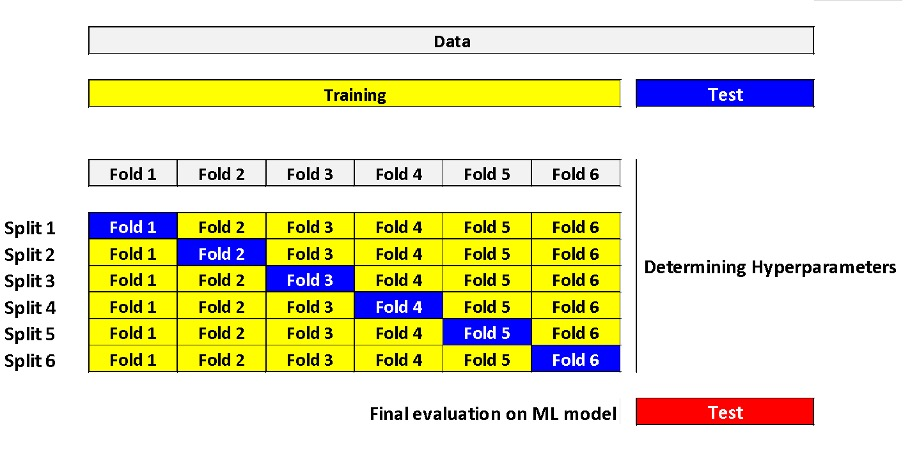
\includegraphics[width=1\textwidth]{images/Cross.jpg}
		\caption{The k-fold cross-validation randomly splits the original dataset into k number of folds\cite{kili}}
		\label{fig:cross}
	\end{center}
\end{figure}

\vspace{-20pt} 

The process works as follows:

\begin{enumerate}
	\item The model is trained on \(k-1\) of the folds and tested on the remaining fold.
	\item This process is repeated \(k\) times, with each fold used as the test set once.
	\item The final performance metric is averaged over all \(k\) trials, giving a more robust estimate of the model's ability to generalize.
\end{enumerate}



In practice, common variations of cross-validation include:
\begin{itemize}
	\item \textbf{k-fold cross-validation:} Typically with \(k = 5\) or \(k = 10\), this method divides the dataset into \(k\) folds and tests the model on each fold.
	\item \textbf{Leave-one-out cross-validation (LOOCV):} Where each data point acts as a single test set.
\end{itemize}

Cross-validation ensures that the model's evaluation is more stable, reliable, and less dependent on any specific train-test split configuration.\cite{kili}

\section{Neural Networks and Deep Learning}

Another artificial intelligence algorithm we will introduce the fundamental concepts is artificial neural networks (ANNs), followed by a deeper dive into deep learning (DL), which is an extension of ANNs.

\subsubsection{Artificial Neural Networks}

\textit{What are Artificial Neural Networks (ANNs)?}

Artificial Neural Networks (ANNs) are computational models inspired by the human brain (see the figure \ref{fig:neuronal}). They consist of interconnected nodes (also called neurons) organized in layers: an input layer, one or more hidden layers, and an output layer. Each node in a layer receives input from the previous layer, processes it, and passes the result to the next layer. The strength of the connection between nodes is determined by weights, which are learned during training.\cite{aiml2024}

\begin{figure}[h!]
	\begin{center}  % Usamos el entorno 'center'
		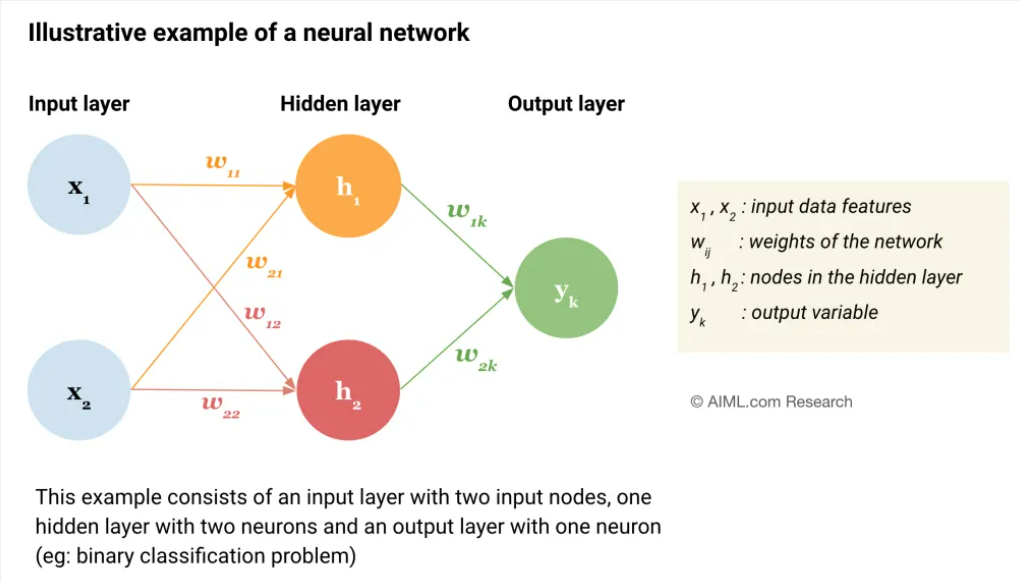
\includegraphics[width=1\textwidth]{images/neuronal.png}
		\caption{A simple neural network, an illustrative example\cite{aiml2024}}
		\label{fig:neuronal}
	\end{center}
\end{figure}

\vspace{-20pt} 


\begin{itemize}
	\item \textbf{Input Layer:} The input layer consists of neurons that receive the raw data and pass it to the hidden layers for further processing.
	\item \textbf{Hidden Layers:} These layers process the input data using activation functions to introduce non-linearity, allowing the model to learn complex patterns.
	\item \textbf{Output Layer:} The output layer produces the final result of the network, whether it's a classification label, continuous value, or probability.
\end{itemize}

ANNs are widely used in machine learning tasks such as classification, regression, and pattern recognition.\cite{aiml2024}

\subsubsection{Deep Learning}

\textit{What is Deep Learning (DL)?}

Is a subset of machine learning that builds upon artificial neural networks by introducing \textbf{deep architectures}. These architectures consist of multiple hidden layers, enabling models to learn complex and hierarchical representations of data. With deep learning, neural networks can automatically learn high-level features from raw data without the need for manual feature extraction. This makes DL particularly powerful in fields like computer vision, speech recognition, and natural language processing.\cite{turing}

The deeper the network (more layers), the more complex patterns it can capture, making deep learning models more capable of handling high-dimensional data and tasks that require advanced feature learning.

\subsubsection{Deep Learning against Neuronal Network}

\textit{What is New in DL Models Compared to Traditional Feedforward Neural Networks?}

Several innovations have contributed to the success of deep learning models compared to traditional feedforward neural networks:\cite{turing}

\begin{itemize}
	\item \textbf{Convolutional Layers:} Used primarily in Convolutional Neural Networks (CNNs), these layers are designed to automatically detect spatial hierarchies in data, such as edges in images, making them highly effective for image classification and recognition tasks.
	\item \textbf{Recurrent Neural Networks (RNNs):} These networks include feedback loops that allow information to persist, making them ideal for sequence data like time series or text, where past inputs influence future predictions.
	\item \textbf{Backpropagation:} A key advancement in neural networks, backpropagation allows for efficient training by adjusting weights based on the error in the output, making it possible to train deeper networks and improve their performance.
	\item \textbf{Other Advancements:} Techniques such as dropout, batch normalization, and the use of GPUs for faster computation have significantly improved the training and performance of deep learning models.
\end{itemize}

These innovations make deep learning models more powerful and flexible compared to traditional feedforward neural networks, allowing them to solve more complex problems and generalize better to unseen data.\cite{turing}

\section{Applications of Deep Learning}

Deep learning has revolutionized many fields, demonstrating transformative results in various domains. Below are two notable case studies where deep learning has produced astonishing results:



\subsection{AlphaFold and Protein Structure Prediction}
AlphaFold, developed by DeepMind, has made significant advances in predicting protein structures. This has been a longstanding challenge in biology, and AlphaFold's ability to predict the 3D structure of proteins based on their amino acid sequences has profound implications for drug discovery and disease research \cite{alphafold2024} (See Figure \ref{fig:alpha}).


In the Figure \ref{fig:alpha}, panel a shows AlphaFold's performance on the CASP14 dataset (n = 87 protein domains) compared to the top 15 entries out of 146, with group numbers assigned by CASP. The data represent the median and 95\% confidence interval, estimated from 10,000 bootstrap samples. Panel b displays our prediction of CASP14 target T1049 (PDB 6Y4F, blue) alongside the true structure (green), excluding four C-terminal residues as B-factor outliers. Panel c shows the accurate prediction of a zinc-binding site in target T1056 (PDB 6YJ1). Panel d illustrates the correct domain packing of the 2,180-residue chain in CASP target T1044 (PDB 6VR4), predicted using AlphaFold without intervention. Panel e depicts the model architecture, with arrows indicating information flow and array shapes specified for sequences (s), residues (r), and channels (c).\cite{alphafoldpaperswithcode}

\begin{figure}[h!]
	\begin{center}  % Usamos el entorno 'center'
		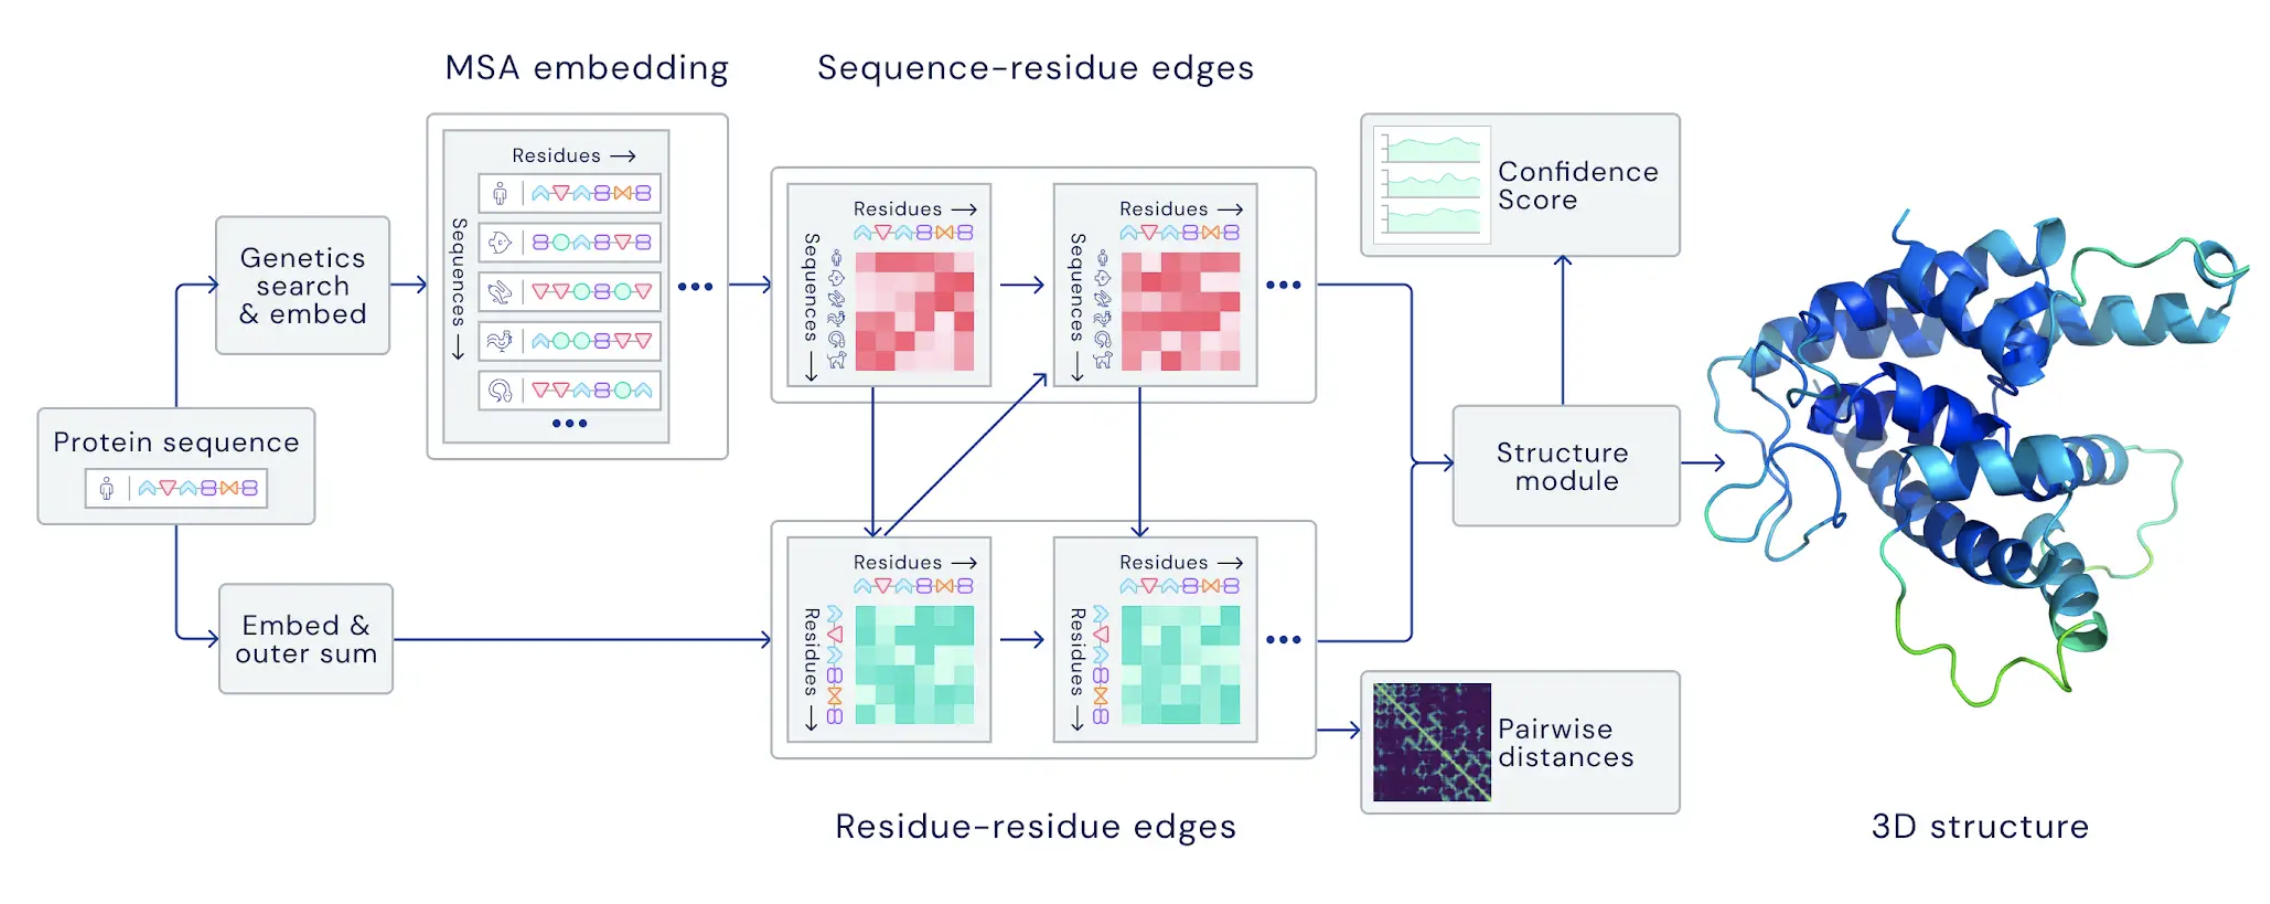
\includegraphics[width=1\textwidth]{images/Alpha.png}
		\caption{Example of AlphaFold\cite{alphafoldpaperswithcode}}
		\label{fig:alpha}
	\end{center}
\end{figure}
\vspace{-11pt}

\subsection{Google’s DeepMind AI in Medical Imaging}
DeepMind's AI has achieved remarkable results in medical imaging, particularly in diagnosing diseases such as diabetic retinopathy and age-related macular degeneration (AMD). By analyzing retinal scans, the AI system matches or exceeds the diagnostic accuracy of expert doctors, aiding in early detection and improving patient outcomes.

In the figure \ref{fig:deep} Training process for a deferral AI model in medical imaging. Medical cases are processed by a \textbf{Predictive AI Model}, producing \textit{predictive confidence scores}. In parallel, a \textbf{Clinical Workflow} provides \textit{retrospective clinician opinions}. These inputs are used to train the \textbf{Deferral AI Model}, which leverages \textit{biopsy-proven ground truth labels} to determine when to defer to human experts based on confidence levels and clinician feedback.
%\vspace{-11pt}

\begin{figure}[h!]
	\begin{center}  % Usamos el entorno 'center'
		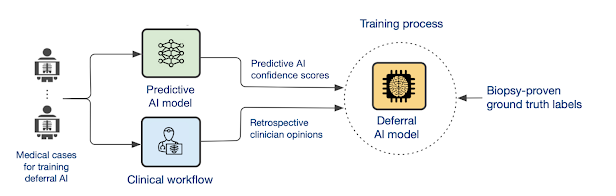
\includegraphics[width=1\textwidth]{images/deepmind.png}
		\caption{Example of AlphaFold\cite{alphafoldpaperswithcode}}
		\label{fig:deep}
	\end{center}
\end{figure}


\section{Challenges in Deep Learning}

Deep learning models face a variety of challenges, two of the most prominent being overfitting and data limitations, especially in specialized fields such as biomedical applications.


\subsection{Overfitting and Mitigation Techniques}

Overfitting is one of the shortcomings in machine learning that hinders the accuracy and performance of the model. occurs when a model learns to perform exceptionally well on the training data, but fails to generalize to unseen data. This happens when the model becomes too tailored to the specific training set, capturing noise and patterns that don't apply to other data. The result is reduced accuracy and performance on real-world data, which undermines the model's effectiveness in practical applications.\cite{overfittingprotecciondatos}

\begin{itemize}
	\item \textbf{Dropout:} A regularization method that randomly disables a fraction of neurons during training, forcing the network to learn more robust features.
	\item \textbf{Regularization:} Techniques like L1 or L2 regularization add penalty terms to the loss function, discouraging the model from fitting excessively to the training data.
	\item \textbf{Early Stopping:} This technique halts training when the model's performance on a validation set starts to degrade, preventing the model from overfitting to the training data.
\end{itemize}

\subsection{Addressing Data Limitations in Biomedical Applications}
In biomedical applications, deep learning models often struggle with limited data. This is especially challenging in fields like medical imaging or genomics, where collecting large, labeled datasets can be costly and time-consuming. Several techniques can help alleviate this issue:

\begin{itemize}
	\item \textbf{Data Augmentation:} This involves creating modified versions of the training data (e.g., rotating, zooming, or flipping images) to increase the dataset's size and diversity, helping the model generalize better.
	\item \textbf{Transfer Learning:} Pretrained models on large datasets are fine-tuned on smaller biomedical datasets, leveraging knowledge learned from a broader task to improve performance on a specific biomedical task.
	\item \textbf{Synthetic Data Generation:} Techniques such as generative adversarial networks (GANs) can be used to generate synthetic data that mimics real-world biomedical data, further expanding the available dataset for training deep learning models.
\end{itemize}


\section{Conclusion}

Validating machine learning models is essential to ensure their accuracy, honesty, and generalizability. A reliable model is one that not only performs well on training data but also generalizes effectively to new, unseen data. Techniques like cross-validation and careful data splitting help in assessing a model's robustness, enabling us to avoid pitfalls like overfitting.

When working with deep learning (DL), while the technology has proven transformative in fields such as healthcare and protein folding, it is far from perfect. The complexity of DL models makes it essential for developers to understand the underlying processes. This knowledge ensures that they can apply appropriate techniques, such as dropout or data augmentation, to avoid overfitting and manage data limitations effectively. Ultimately, the success of DL models relies on a careful balance between model complexity, data quality, and proper validation.

\section{Repository Github}
Further information, including the source code and full project documentation, can be accessed through the GitHub repository.  \href{https://github.com/Diegodepab/Supervised_Learning_Model_Evaluation_Metrics}{Click here to go to the repository.} 



\bibliographystyle{plain}  % Puedes cambiar "plain" por el estilo de tu preferencia, como apalike, ieeetr, etc.
\bibliography{bibliography}  % Aquí va el nombre de tu archivo .bib (sin la extensión .bib)
\end{document}
